\chapter{Literature Survey}

\section{Paper Analysis}
For our platform to form we had to take assistance from already explored thesis and paper.They provided us with basic understanding and different aspects of interpretation of modern traffic problem.The guides we used to expand our platform includes.

\begin{figure}[htb]
    \centering
    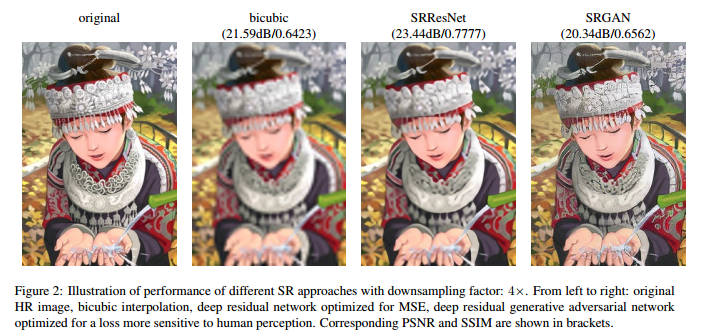
\includegraphics[width=\linewidth]{srdiff.jpg}
    \caption{Better edge correction}
    \label{fig:srdiff} % insert suitable label, this is used to refer to a fig from within the text
\end{figure}

Deep Learning-based methods are currently active and showing significant performances on SISR tasks. Super-Resolution Convolutional Neural Network (SRCNN) is the method proposed at this very early stage. C. Dong et al.use 2 to 4 CNN layers to prove that the learned CNN layers model performs well on SISR tasks. The authors concluded that using a larger CNN filter size is better than using deeper CNN layers. SRCNN is followed by Deeply-Recursive Convolutional Network for Image Super-Resolution (DRCN). DRCN uses deep (a total of 20) CNN layers, which means the model has huge parameters. However, they share each CNN’s weight to reduce the number of parameters to train, meaning they succeed in training the deep CNN network and achieving significant performances. The other Deep Learning based method VDSR is proposed by the same authors of DRCN. VDSR uses Deep Residual Learning, which was developed by researchers from Microsoft Research and is famous for receiving first place in ILSVRC 2015 (a large image classification competition). By using residual-learning and gradient clipping, VDSR proposed away of significantly speeding up the training step. Very deep Residual Encoder-Decoder Networks(RED) are also based on residual-learning. RED contains symmetric convolutional(encoder) and deconvolutional(de-coder)layers. It also has skip connections and connects instead to every two or three layers. Using this symmetric structure, they can train very deep (30 of) layers and achieve state-of-the-art performance. These studies therefore reflect the trendof “the Deeper the Better”. Onthe other hand, Yaniv Romano et al. proposed Rapid and Accurate Image Super Resolution (RAISR) , which is a shallow and faster learning-based method. It classifies input image patches according to the patch’s angle, strength and coherence and then learn maps from LR image to HR image among the clustered patches. C. Dong et al. also proposed FSRCNN as a faster version of their SRCNN .FSRCNN uses transposed CNN to process the input image directly. RAISR and FRSCNN’s processing speeds are 10 to 100 times faster than other state-of-the-art Deep Learning-based methods. However, their performance is not as high as other deeply convolutional methods,like DRCN, VDSR orRED.

\subsection{Fast and Accurate Image Super Resolution by Deep CNN with Skip Connection and Network in Network}
In this paper the authors propose a highly efficient and faster Single Image Super Resolution (SISR) model with Deep Convolutional neural networks (Deep CNN) . Deep CNN have recently shown that they have a significant reconstruction performance on single image super resolution. The current trend is using deeper CNN layers to improve performance . However , deep models demand larger computation resources and are not suitable for network edge devices like mobile, tablet and IoT devices . Our model achieves state of the art reconstruction performance with at least 10 times lower calculation cost by Deep CNN with Residual Net, Skip Connection and Network in Network (DCSCN) . A combination of Deep CNNs and Skip connection layers are used as a feature extractor for image features on both local and global areas . Parallelized 1x1 CNN s, like the one called Network in Network , are also used for image reconstruction . That structure reduces the dimensions of the previous layer ’s output for faster computation with less information loss , and make it possible to process original images directly . Also w e optimize the number of layers and filters of each CNN to significantly reduce the calculation cost . Thus, the proposed algorithm not only achieves state of the art performance but also achieve s faster and more efficient computation .

\begin{figure}[htb]
    \centering
    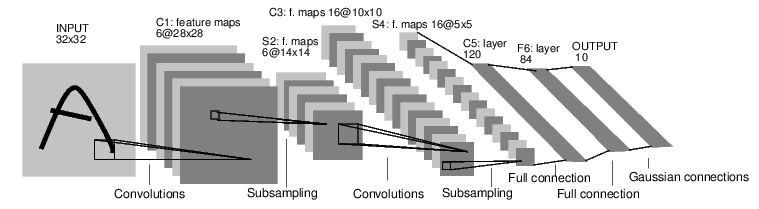
\includegraphics[width=\linewidth]{fe.png}
    \caption{Feature Extraction}
    \label{fig:fe} % insert suitable label, this is used to refer to a fig from within the text
\end{figure}

\subsection{Photo-Realistic Single Image Super-Resolution Using a Generative Adversarial Network}
Despite the breakthroughs in accuracy and speed of single image super-resolution using faster and deeper con- volutional neural networks, one central problem remains largely unsolved: how do we recover the finer texture details when we super-resolve at large upscaling factors? The behavior of optimization-based super-resolution methods is principally driven by the choice of the objective function. Recent work has largely focused on minimizing the mean squared reconstruction error. The resulting estimates have high peak signal-to-noise ratios, but they are often lacking high-frequency details and are perceptually unsatisfying in the sense that they fail to match the fidelity expected at the higher resolution. In this paper, the authors introduce SRGAN, a generative adversarial network (GAN) for image super- resolution (SR). To our knowledge, it is the first framework capable of inferring photo-realistic natural images for 4 × upscaling factors. To achieve this, we propose a perceptual loss function which consists of an adversarial loss and a content loss. The adversarial loss pushes our solution to the natural image manifold using a discriminator network that is trained to differentiate between the super-resolved images and original photo-realistic images. In addition, they use a content loss motivated by perceptual similarity instead of similarity in pixel space. The deep residual network is able to recover photo-realistic textures from heavily downsampled images on public benchmarks. An extensive mean-opinion-score (MOS) test shows hugely significant gains in perceptual quality using SRGAN. The MOS scores obtained with SRGAN are closer to those of the original high-resolution images than to those obtained with any state-of-the-art method.

\subsection{Image Super-Resolution Using Deep Convolutional Networks}
They propose a deep learning method for single image super-resolution (SR). Their method directly learns an end-to-end mapping between the low/high-resolution images. The mapping is represented as a deep convolutional neural network (CNN) that takes the low-resolution image as the input and outputs the high-resolution one. They further show that traditional sparse-coding-based SR methods can also be viewed as a deep convolutional network. But unlike traditional methods that handle each component separately, our method jointly optimizes all layers. Their deep CNN has a lightweight structure, yet demonstrates state-of-the-art restoration quality, and achieves fast speed for practical on-line usage. They explore different network structures and parameter settings to achieve trade-offs between performance and speed. Moreover, they extend our network to cope with three color channels simultaneously, and show
better overall reconstruction quality.
